\documentclass[a4paper,10pt]{article}
\usepackage[utf8]{inputenc}
\usepackage{todonotes}
\usepackage{fullpage}
\usepackage{graphicx}
\usepackage{float}
\usepackage{multirow}
\usepackage{wrapfig,booktabs}
\usepackage{tikz}
\usepackage{circuitikz}
\usepackage{cite}
\usepackage{tikz-timing}
\usepackage{url}
\usepackage{hyperref}
\usepackage{subcaption}
\hypersetup{
    colorlinks,
    citecolor=black,
    filecolor=black,
    linkcolor=black,
    urlcolor=black
}

\usepackage{pgf}
\usetikzlibrary{arrows,automata}
\usetikzlibrary{patterns}
\usetikzlibrary{shapes.geometric}
\usetikzlibrary{fit}
\usetikzlibrary{calc}
\usetikzlibrary{intersections}
\usetikzlibrary{backgrounds}
\usetikzlibrary{arrows, decorations.markings}
\usetikzlibrary{decorations.pathreplacing}
\usetikzlibrary{automata} %state machine stuff
\usetikzlibrary{positioning} %midway
\tikzstyle{vecArrow} = [thick, decoration={markings,mark=at position
   1 with {\arrow[semithick]{open triangle 60}}},
   double distance=1.4pt, shorten >= 5.5pt,
   preaction = {decorate},
   postaction = {draw,line width=1.4pt, white,shorten >= 4.5pt}]
\tikzstyle{module} = [rectangle, minimum width = 2 cm,minimum height = 2 cm, draw]

%opening
\title{Brick sorter}
\author{Nikolaj Iversen, Matthias Harald Hessels}


%Todo notes
\usepackage{nameref}
\makeatletter
\newcommand*{\currentname}{\@currentlabelname}
\makeatother

\newcommand{\nikolaj}[1]{\todo[inline,color=red!20,author=Nikolaj]{\currentname: ~ #1}}
\newcommand{\matthias}[1]{\todo[inline,color=blue!20,author=Matthias]{\currentname: ~ #1}}

\newcommand{\figscale}{0.8}

\usepackage{diagbox}
\usepackage{amsmath}
\begin{document}

\begin{titlepage}
	\centering
	{\scshape\LARGE University of Southern Denmark \par}
	\vspace{1cm}
	{\scshape\Large Embedded Programming (EMB1) \par}
	\vspace{1.5cm}
	{\huge\bfseries Brick Sorter\par}
	\vspace{2cm}
	{\Large\itshape Group 3 \\ Nikolaj Iversen \{nive12\} \\ \& \\ Matthias Harald Hessels \{mahes12\} \par}
	\vspace{1cm}
	\centering
	
\includegraphics[width=0.5\textwidth]{img/sdu}\par
	\vfill
	supervised by\par
	Jørgen Christian Larsen \& Richard Beck
	\vfill

% Bottom of the page
	{\large \today\par}
\end{titlepage}

\tableofcontents
\listoftodos
\thispagestyle{empty}
\addtocounter{page}{-1}
\newpage

\section{Introduction}
In this project a the design of a rotating clock is described.
Using a series of LEDs, mounted on a PCB which rotates, the system will display what would look like the dial on a watch.
The system will be controlled by an FPGA, which is in a fixed position.

% This project is about creating a watch, using a LED strip mounted on a pcb, that then rotates, creating the sense that the watch dial is fixed. 
Since change in images appears smooth after around 30 Hz \cite{article:rpm}, the goal is to get the PCB to rotate with at least 30 RPS.
To estimate the speed of the rotating arm, the arm will be equipped with a magnet and the position is estimated by meassuring the Hall effect on sensors on the ground.
One of the biggest challenges of the project is to get a stationary FPGA to control a rotating board with LEDs.
A custom slip ring is made to deal with this problem.

% \nikolaj{More detail}


\section{Electronics}
\subsection{Power supply}
One of the tasks of the project was to create a power supply for the FPGA board and the external components. This supply should take in a 15 V signal and divide it into 3 different voltage levels which can be seen in table \ref{tab::power_req}. The power supplys should be soldered on a PCB made using Eagle, a CAD program for circuit design. The schematic of the board can be seen on figure \ref{fig::sch_power}.
\subsubsection{Regulators}
\begin{wraptable}{r}{7cm}
 \vspace{5 pt}
 \begin{tabular}{cccc}
  Voltage & Current & Tolerance      & Efficiency \\ \toprule
  12 V    & 1.0 A   & -              & -          \\
  6 V     & 1.5 A   & -              & -          \\
  5 V     & 0.5 A   & $\pm\ 1.5 \%$  & 80\%       \\
  \bottomrule
 \end{tabular}
\caption{Voltage and current requirements for the power supply.}
\label{tab::power_req}
 \vspace{5 pt}
\end{wraptable}
The 5V supply, driving the FPGA, has a requirement to the efficiency which means a switching regulator must be used for this task. 
For the switching regulator a LM2574N-5.0 was chosen as it provides a 0.5A, 5.0V supply.
According to the datasheet, the typical efficiency is 77\%.
\footnote{LM2574N datasheet, p4}
The specified tolerance is 4\% which means the tolerance is worse than required. Further testing is required to see if the configuration is good enough for the application.
\footnote{LM2574N datasheet, p1}
The schematic was designed following the typical application guidelines in the datasheet.
The diode was selected as 1N5817. 
\footnote{LM2574N datasheet, p17}
The $C_{out}$ capacitor was chosen to be $330\mu f$ to minimize ripple voltage.
\footnote{LM2574N datasheet, p19}
Given the input voltage of 15 V and the max current drawn, $0.5 A$, the value of the inductor should be 330 $\mu H$. 
\footnote{LM2574 datasheet p 14, fig 26}
The schematic for the 5 V supply can be seen in figure \ref{fig::sch_power_5V}.

There is no requirements to the efficiency of the 6 and 12 V supplys so a linear regulator is used.
The maximum current in the 6 V supply is 1.5 A, which means a bigger diode is needed.
For this a 1N5408 is chosen, which can deliver an average 3.0 A forward current.
\footnote{1N5408 datasheet, p1}
The capacitors are there to eliminate voltage spikes from the load. A capacitance of $0.1 \mu F$ is chosen.
\footnote{Ref to Practical Electronics page 702}
The schematics of the 6 and 12 V supplys can be seen in figure \ref{fig::sch_power_6V} and \ref{fig::sch_power_12V}.

\begin{figure}[H] %left, bot, right, top
\centering
\begin{subfigure}{0.3\linewidth}
\centering
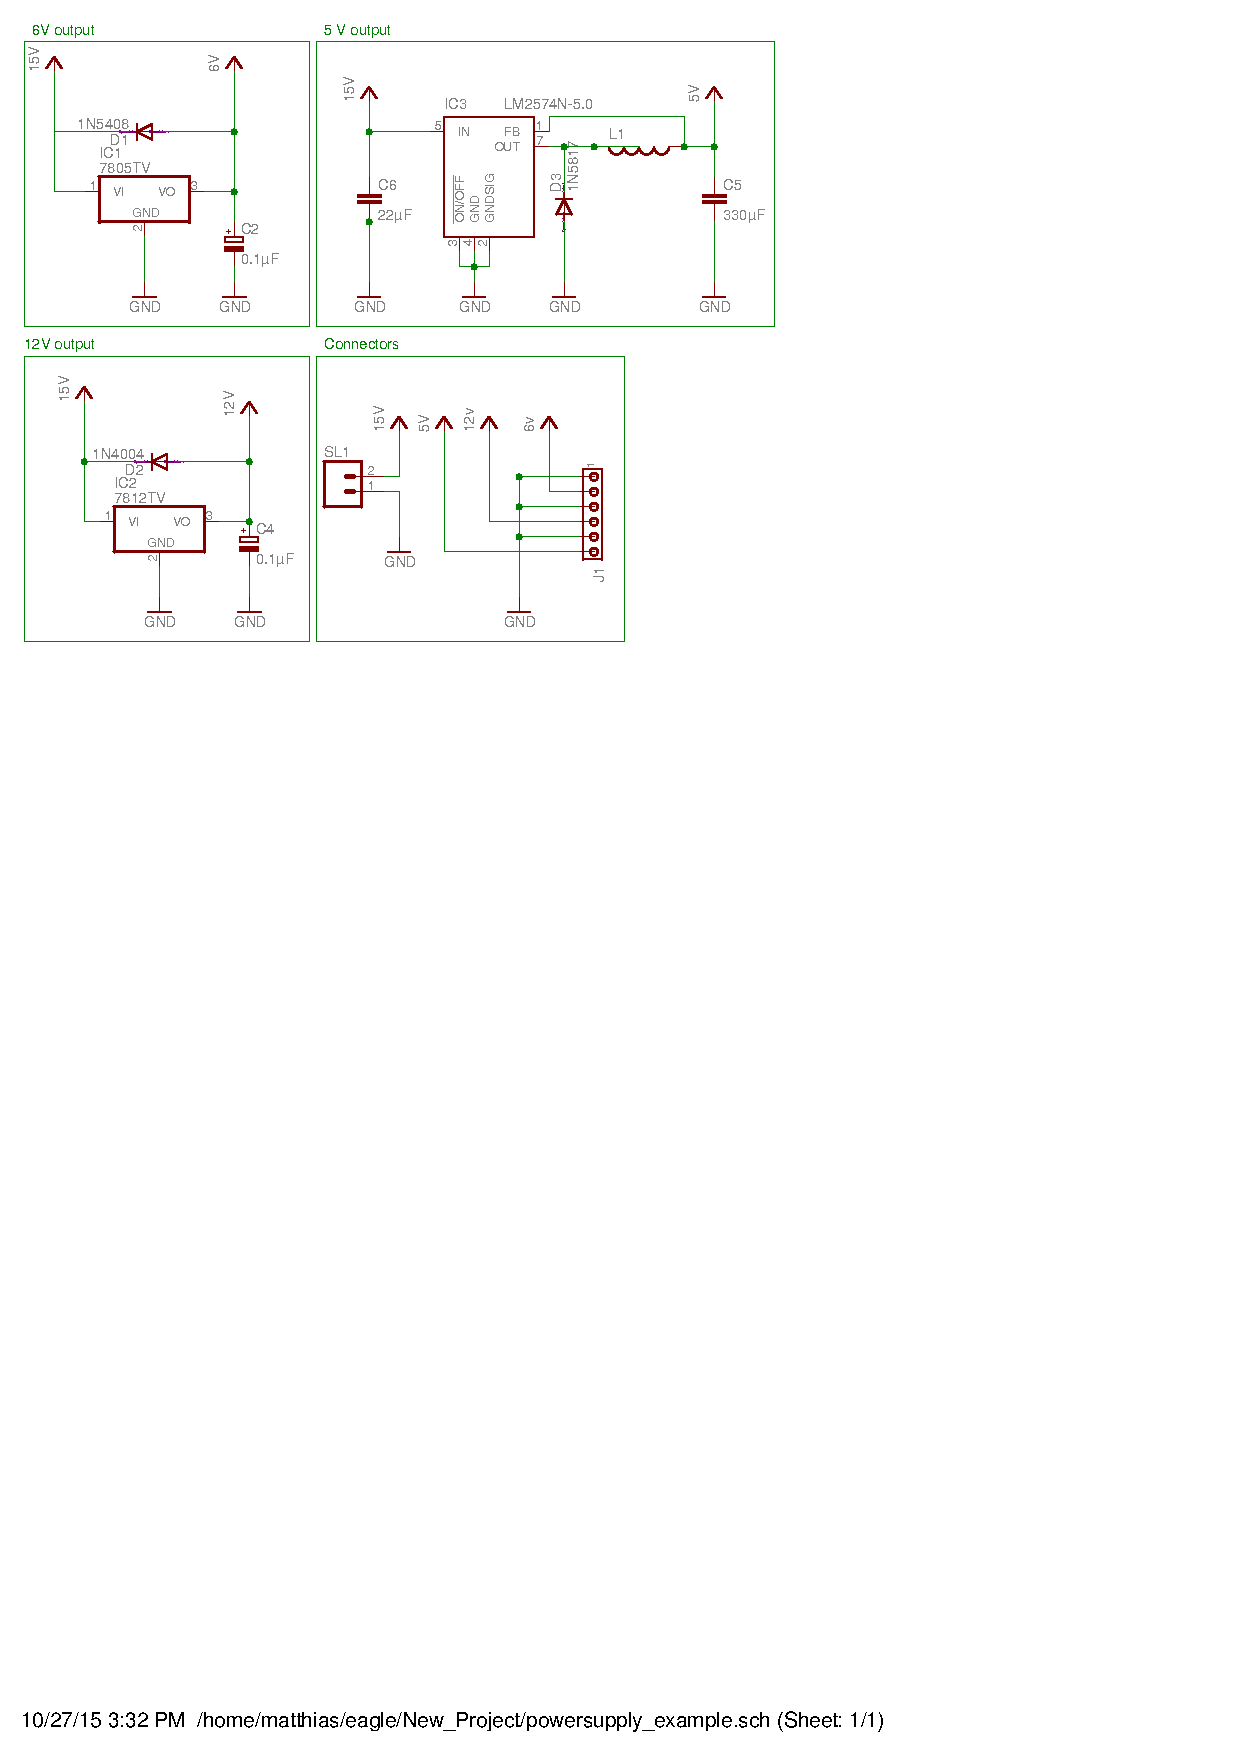
\includegraphics[scale=0.8,trim={0 24cm 15.7cm 0.6cm},clip]{img/powersupply.pdf}
\caption{6V supply.}
\label{fig::sch_power_6V}
\end{subfigure}
\begin{subfigure}{0.4\linewidth}
\centering
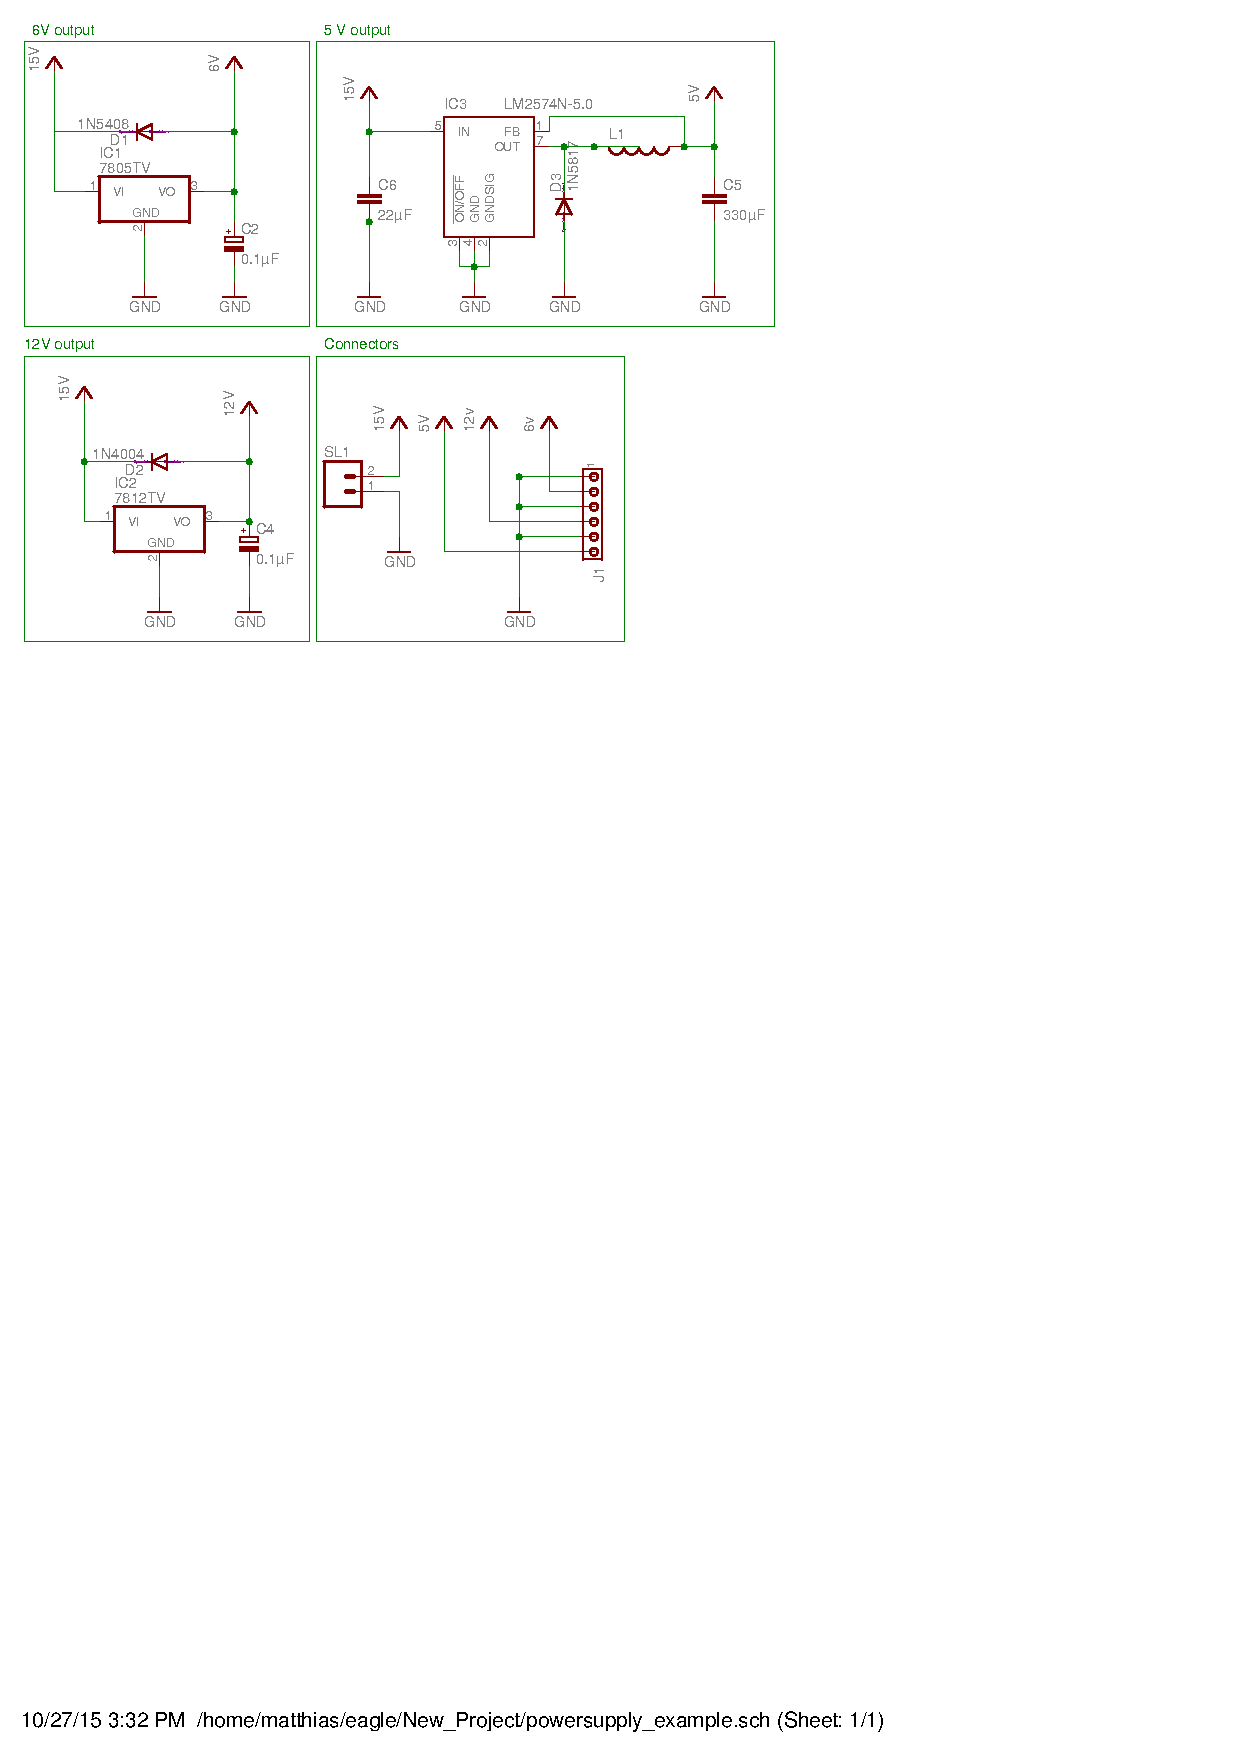
\includegraphics[scale=0.8,trim={5.3cm 24cm 7.8cm 0.6cm},clip]{img/powersupply.pdf}
\caption{5V supply.}
\label{fig::sch_power_5V}
\end{subfigure}

\begin{subfigure}{0.3\linewidth}
\centering
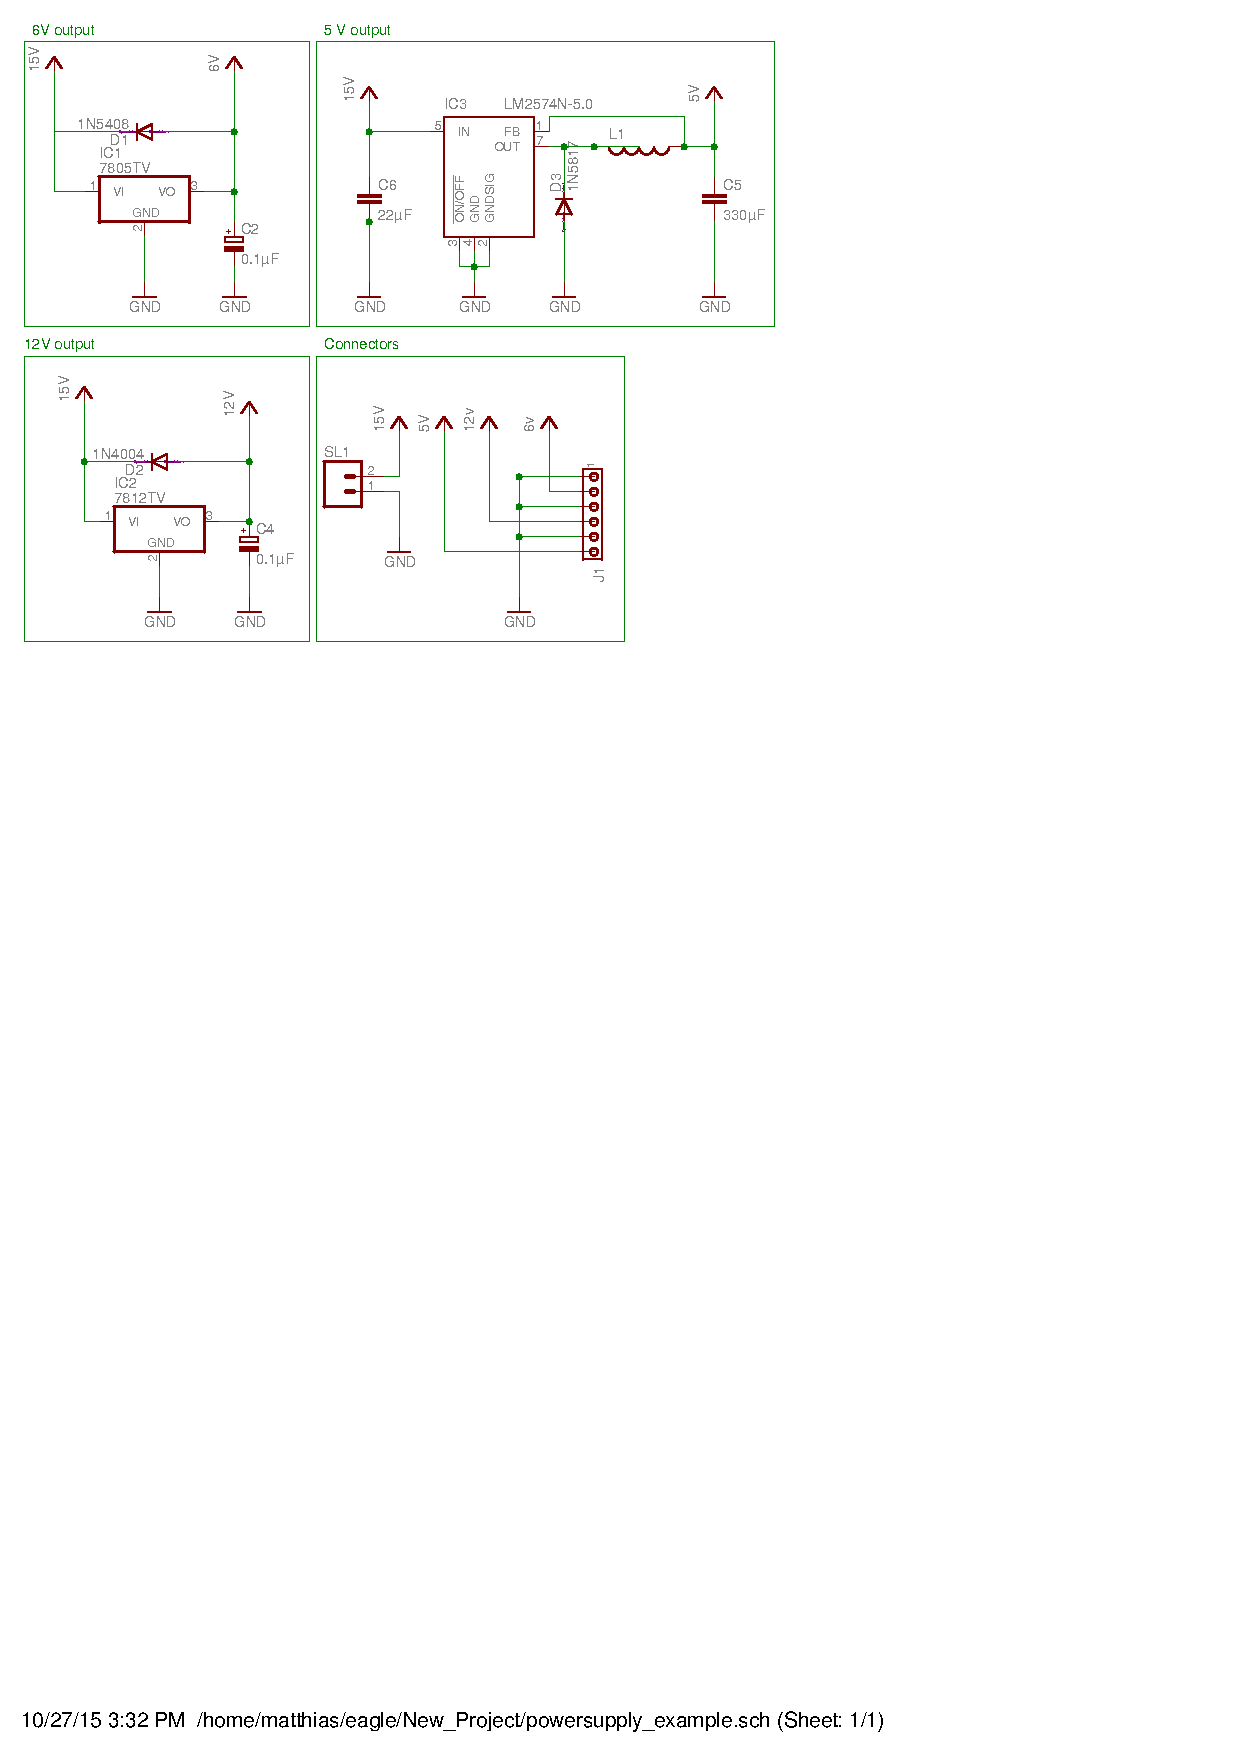
\includegraphics[scale=0.8,trim={0 18.5cm 15.7cm 6.0cm},clip]{img/powersupply.pdf}
\caption{12V supply.}
\label{fig::sch_power_12V}
\end{subfigure}
\begin{subfigure}{0.4\linewidth}
\centering
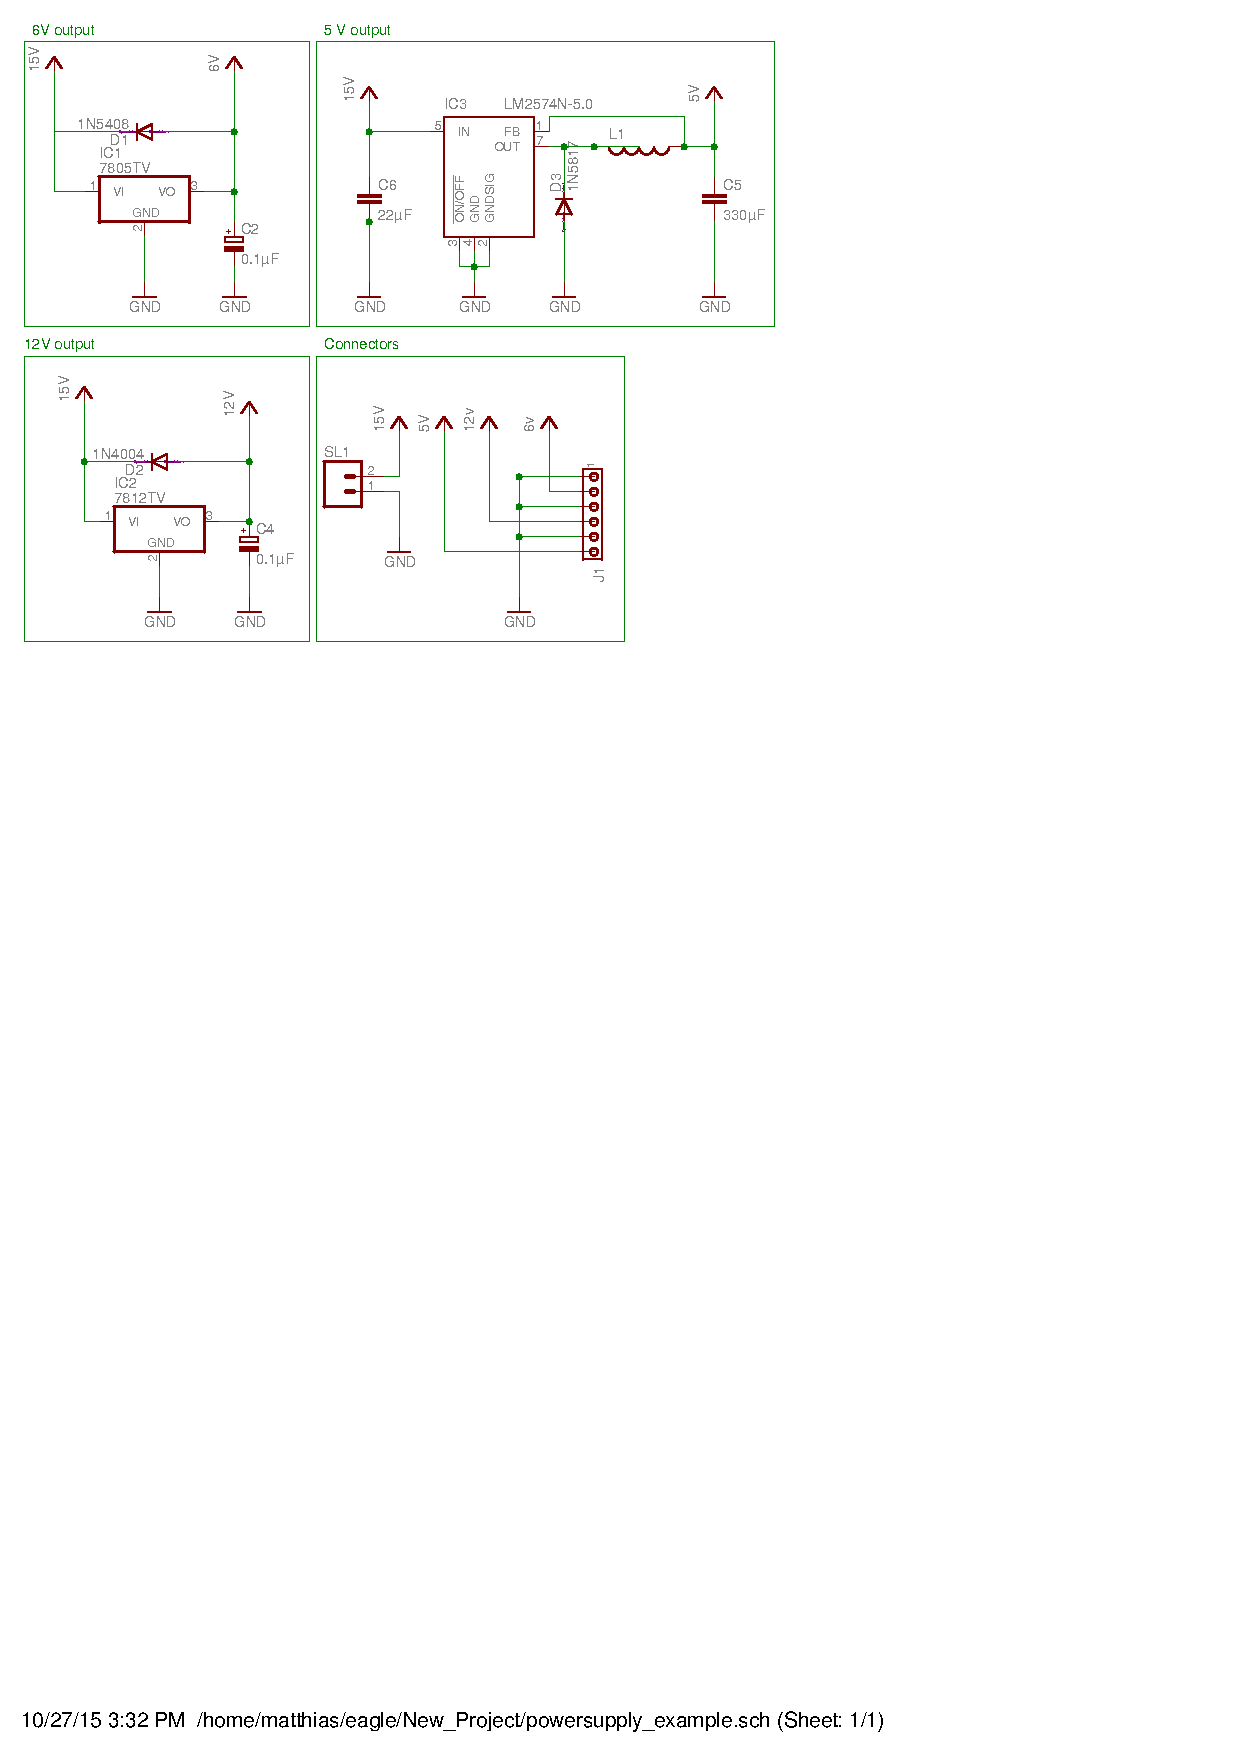
\includegraphics[scale=0.8,trim={5.3cm 18.5cm 10.4cm 6.0cm},clip]{img/powersupply.pdf}
\caption{Breakout pins.}
\label{fig::sch_power_pins}
\end{subfigure}
\caption{Schematic diagram of power supply}
\label{fig::sch_power}
\end{figure}

\subsubsection{Heat}
One of the problems when designing the circuit, is that the linear regulators.
The energy used in the regulator is converted into heat.
The worst case power dissipation can be calculated in equation \ref{eq:pd6} and \ref{eq:pd12}.
\begin{eqnarray}
pD_{6}  =& (15V - 6V) \cdot 1.5A\ &=\ 13.5\ W \label{eq:pd6}\\
pD_{12} =& (15V - 12V)\cdot 1.0A\ &=\ 3\ W \label{eq:pd12}
\end{eqnarray}
The junction to ambient resistance ($R_{ja}$) is $50^\circ C/W$%
\footnote{L7806CV datasheet, p7}
\footnote{LM7812C datasheet, p3}
This means the temperature rise can be calculated in equation \ref{eq:tr6} and \ref{eq:tr12}.
\begin{eqnarray}
T_{r6}  =&  13.5 \cdot 50   &= 675^\circ C \label{eq:tr6}\\
T_{r12} =&  3 \cdot 50      &= 150^\circ C \label{eq:tr12}
\end{eqnarray}
The maximum junction temperature is 150 for the LM7812\footnote{LM7812C p3} and 125 for the L7806CV\footnote{L7806CV, p7}, meaning the temperature for the 12 V supply is close to the maximum and the temperature for the 6 V supply is above.
It is decided to use a heatsink on both.
\matthias{Beskrive forhold ved belastning efter heat sinks er sat på.}
\matthias{Lav nye test af powersupply}

\subsubsection{PCB design}
The components described above, put together as seen in the block diagram in figure \ref{fig::sch_power}. 
% One of the things that were taken into account when designing the PCB was, in order to save space, instead of having one capacitor on the each of the regulator input, the 15V input was put roughly in the middle of the regulators with only one input capacitor
The 15 V input was put between the regulators with only one input capacitor to save space.
A ground plane was added to reduce the resistance to ground.
This has the added benefit that it will be easier to route and faster to produce as less copper is removed.
The pcb can be seen in figure \ref{fig::pcb_power}

\begin{figure}
\centering
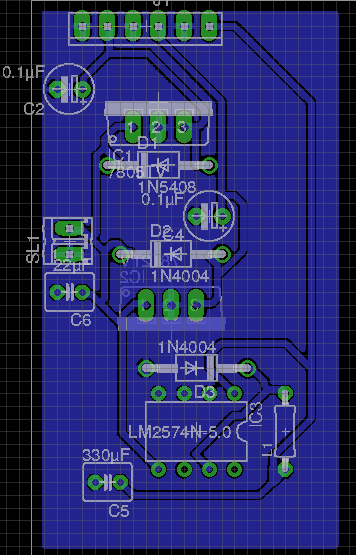
\includegraphics[scale=0.5]{img/pcb_power.png}
\caption{PCB design of the power supply made in Eagle} 
\label{fig::pcb_power}
\end{figure}
\nikolaj{Update figure}

\subsection{Color detection}
In order to detect colors a block gets shined upon with different colored LEDS.
A photo diode will give a voltage linear to the absorbed light.
This voltage will be converted to a digital signal the PFGA can work with.
In this section these modules will be described.
\subsubsection{High Power Diodes}
In order to get maximum brightness, high power diodes are used.
A diode in red, green and blue is used in order to detect different color LEGO blocks.
NTD5867NL mosfet was used to turn the diodes on and off.

The Forward voltage on the red is 1.9 V and 3.2 V for the green and blue LED.
\footnote{led\_datasheet, p5}
The current is chosen at $50 mA$, based on the recommended range for 100\% duty cycle.
\footnote{led\_application\_notes, p2}
\begin{eqnarray}
 R_{red} =& \frac{12-1.9}{0.05} =& 202 \Omega\\
 R_{green} = R_{blue} =& \frac{12-3.2}{0.05} =& 176 \Omega
\end{eqnarray}
The green and blue LEDS are only turned on for a short amount of time so $R_{green}$ and $R_{blue}$ is rounded down to $160 \Omega$.
The $R_{red}$ is rounded down to $200\Omega$.
The schematic can be seen in figure \ref{fig:sch_led}.
A pull down resistor at is used so the FPGA has to deliver a current to turn the mosfet on.

\begin{figure}[h]
\centering
%  \includegraphics[scale =0.8, trim={0,0,0,0},clip]{img/sch_led}
  \caption{Schematic for LEDS.}
  \label{fig:sch_led}
\end{figure}

\subsubsection{Photo Diode}
The photo diode works by producing a current proportional to the light intensity it receives.
To turn this into a voltage readable by the ADC, an opamp is used.
Measurements done by holding a colored LEGO brick up to the same color light source revealed that the current, produced from the photo diode was $5-20 \mu A$.
Tests using a flashlight directly pointed at the photo diode showed that the current could get up to $40 \mu A$.
The desired output should be $0-3.3 V$, same as the logic level used on the FPGA.
If $20 \mu A$ should correlate to $2 V$, the resistor should be $100K\Omega$. 
This gives room for more intensity, so saturation of the op amp less likely with a false positive.

The LM358 is chosen for the op amp.
It can be used with a single supply, but does not have rail to rail output.
Measurements of the output shows that with a supply of 3.3 V the output can vary from 0.05 V to 2.1 V.
Thus a supply of 4.5 V is chosen so the op amp can provide an output ranging from 0.05 to 3.3 V, thus creating a pseudo rail to rail.
To get a 4.5 V supply, a voltage divider is used. This is done with 3 resistors so there is a 3.3 V supply for the ADC and a 4.5 V supply for the op amp.
The schematic for the photo diode can be seen in figure \ref{fig:sch_photo_diode}.

The MCP3001 is an ADC in a single component.
It provides a 10 bit variable, sent over SPI.
The supply is chosen to be 3.3 V, keeping the logic level the same as the FPGA.

\begin{figure}[h]
\centering
%  \includegraphics[scale =0.8, trim={0,0,0,0},clip]{img/sch_photo_diode}
  \caption{Schematic for photo diode.}
  \label{fig:sch_photo_diode}
\end{figure}


\newpage

\section{VHDL}
The VHDL code has been split up into small modules in order to heighten the level of abstraction, and to make it possible to reuse the code in other projects. 
The modules are as following; A top module that connects the different components, a module for serial communication with the ADC, a driver for the LED's, a PWM generator for the servo and a serial communicator to the PC using $\mu$TosNet.
\subsection{Top Module}
This module is only there in order to take the different components and put them together in order to make the application. This is done using components and port maps. A block diagram of the components used and how the internal signals are structured can be seen in figure \ref{fig::block_dia}.
\begin{figure}[h]
\centering
 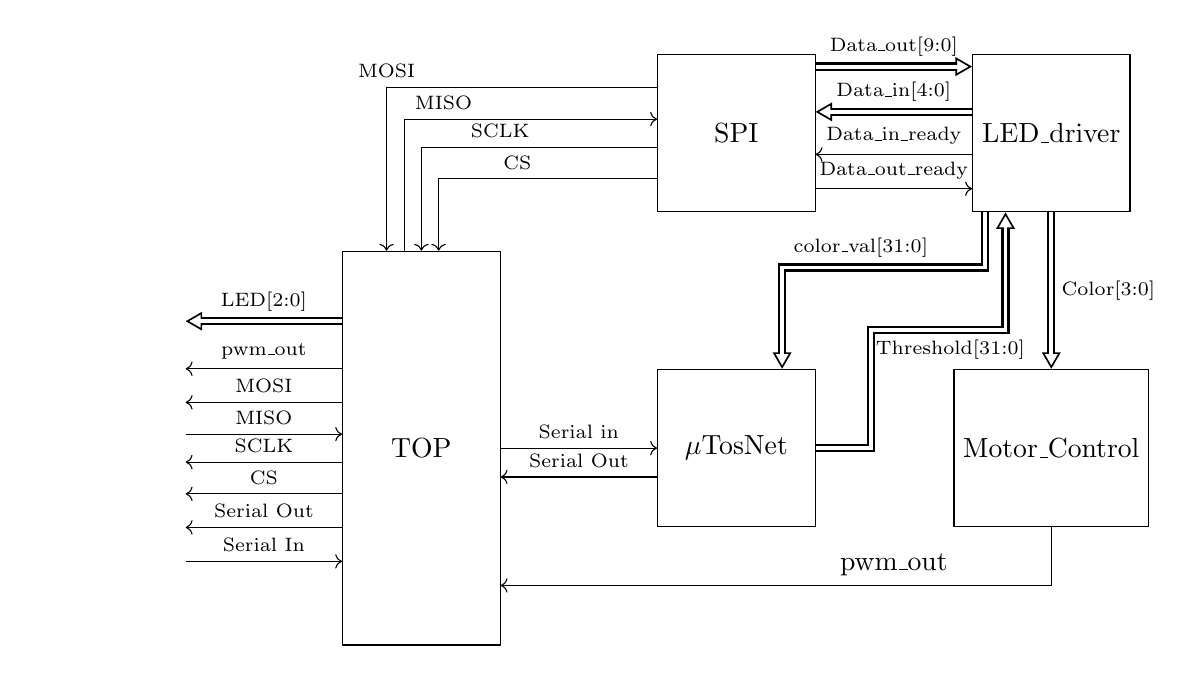
\begin{tikzpicture}[node distance=4 cm]
 
 \node[module,minimum height= 5 cm,name=top] {TOP};
 \node[module,name=tosnet,right of = top] {$\mu$TosNet};
 \node[module,name=spi, above of = tosnet] {SPI};  
 \node[module,name=led_control, right of = spi] {LED\_driver};
 \node[module,name=motor,right of = tosnet] {Motor\_Control};
 \node[rectangle,minimum width = 2 cm, minimum height = 5 cm,name=empty, left of = top] {};
                      
 \draw[<-] (top.100) |- node[anchor=south]{\scriptsize MOSI}  (spi.150);
 \draw[->] (top.95)  |- node[anchor=south,xshift=0.5cm]{\scriptsize MISO} (spi.170);
 \draw[<-] (top.90)  |- node[anchor=south,xshift=1cm]{\scriptsize SCLK} (spi.190);
 \draw[<-] (top.85)  |- node[anchor=south,xshift=1 cm]{\scriptsize CS}   (spi.210);

 \draw[vecArrow] (top.122) to node[anchor=south]{\scriptsize LED[2:0]}  (empty.58);
 \draw[->] (top.135) to node[anchor=south]{\scriptsize pwm\_out}  (empty.45);
 \draw[->] (top.150) to node[anchor=south]{\scriptsize MOSI}  (empty.30);
 \draw[<-] (top.170) to node[anchor=south]{\scriptsize MISO} (empty.10);
 \draw[->] (top.190) to node[anchor=south]{\scriptsize SCLK} (empty.350);
 \draw[->] (top.210) to node[anchor=south]{\scriptsize CS}   (empty.330);
 \draw[->] (top.225) to node[anchor=south]{\scriptsize Serial Out}   (empty.315);
 \draw[<-] (top.235) to node[anchor=south]{\scriptsize Serial In}   (empty.305);
 
 \draw[vecArrow] (spi.40) to node[anchor=south]{\scriptsize Data\_out[9:0]} (led_control.140);
 \draw[vecArrow] (led_control.165) to node[anchor=south]{\scriptsize Data\_in[4:0]} (spi.15);
 \draw[<-] (spi.345) to node[anchor=south]{\scriptsize Data\_in\_ready} (led_control.195);
 \draw[->] (spi.325) to node[anchor=south]{\scriptsize Data\_out\_ready} (led_control.215);
 
 \draw[vecArrow] (led_control) to node[anchor=west]{\scriptsize Color[3:0]} (motor); 
 \draw[->] (tosnet.200) to node[anchor = south]{\scriptsize Serial Out} (top.340);
 \draw[->] (top.east) to node[anchor = south] {\scriptsize Serial in} (tosnet.west);
 \draw[->] (motor) |- node[anchor = south,xshift=-2 cm]{pwm\_out} (top.300);
 
 \draw[vecArrow] (tosnet.east) to ++(0.7,0) to ++(0,1.5) -| node[anchor=north,xshift=-0.7cm]{\scriptsize Threshold[31:0]} (led_control.240);
 \draw[vecArrow] (led_control.230) to ++(0,-0.7) -| node[anchor=south,xshift=1cm]{\scriptsize color\_val[31:0]} (tosnet.60);
 
 \end{tikzpicture}
 \caption{Block diagram of the system}
 \label{fig::block_dia}
\end{figure}


\subsection{LED\_driver}
This module is the brain of the project. This is where it is decided which LED should be on at the given moment, it takes the samples from the ADC, it analyzes the results of the ADC and decides which color the brick is.

\subsubsection{Implementation}
In order to make this work a state machine is implemented. A state diagram can be seen figure \ref{fig::state_led}. It starts in in idle state. In this state the red LED is turned on, and a sample from the ADC is done. If this value is bigger than a specific threshold, which mean that a brick is present at the photo diode. The state is then changed and the different LED's are flashed one at a time, and the value of the photo diode is read from the ADC. Instead of just taking one sample of each color, it was chosen to take a number of samples and take the mean in order to ensure that the choice is more reliable. In order to make the mean calculation easier, the number of samples should be a power of 2, since division with a power of 2 is just right shifting the number of times of the power, so 4 samples = 2 $\times$ rightshift. This is what is happening in the Decider state in figure \ref{fig::state_led}, note sample\_count is a counter that counts run-throughs, and not individual colors. When the decider detects a color, i.e the ADC value is bigger than a specified threshold, a bit is set in a signal corresponding to the given color. The thresholds of the colors can be updated from the computer through $\mu$TosNet. 

\matthias{Skriv om til Nearest Neighbor implementering}

\begin{figure}[h]
\centering
 \begin{tikzpicture}[node distance=2.5cm]
 
 \node[circle,minimum width = 7 cm,name = c]{};
 \node[accepting,state,	name=state0, minimum width = 1.3 cm] at (c.90)    {Idle}; 
 \node[square,name=start,above of = state0,yshift=-1.2 cm]                {Start};
 \node[state,name=stateR, minimum width = 1.3 cm]            at (c.18)    {Red};
 \node[state,name=stateG, minimum width = 1.3 cm]            at (c.-56)   {Green};
 \node[state,name=stateB, minimum width = 1.3 cm]            at (c.234)   {Blue};
 \node[state,name=decide, minimum width = 1.3 cm]            at (c.162)   {Decider};
 
 \draw[->] (state0)   edge[bend left=27] node[midway,above,fill=white,xshift=0.9cm,yshift=-0.5cm] {ADC data $>$ threshold}  (stateR);
 \draw[->] (stateR)   edge[bend left=27] node[midway,fill=white]                                  {dummy\_count $=$ 2}            (stateG);
 \draw[->] (stateG)   edge[bend left=27] node[midway,below]                                       {dummy\_count $=$ 2}            (stateB);
 \draw[->] (stateB)   edge[bend left=27] node[midway,fill=white]                                  {dummy\_count $=$ 2}            (decide);
 \draw[->] (decide)   edge[bend left=27] node[midway,below,fill=white]                            {sample\_count $=$ 4}     (state0);
 \draw[->] (decide)   to                 node[midway,above]                                       {sample\_count $!=$ 4}    (stateR);
 \draw[->] (start)    to                                                                                                    (state0);
 
 \end{tikzpicture}
 \caption{State machine of \textbf{LED\_driver}}
 \label{fig::state_led}
\end{figure}

\subsubsection{Extra considerations}
One of the things that was thought of during implementation the Nearest Neighbor algorithm was whether or not there was logic enough in order to contain all of the data needed without using external memory. In the beginning a simpler algorithm was implemented, that uses thresholds in order to decide which color brick there is.

\begin{figure}[H]
 \centering
\setlength{\belowcaptionskip}{5pt}

\begin{subfigure}[b]{0.70\textwidth}
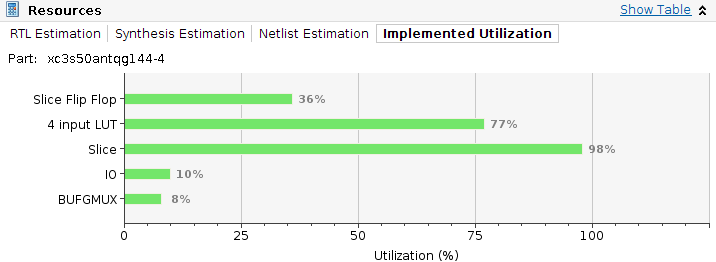
\includegraphics[width=\linewidth]{img/nearest_neighbor.png}
\caption{Logic consumption of the project with Nearest Neighbor algorithm as decider}
\end{subfigure}

\begin{subfigure}[b]{0.70\textwidth}
\centering
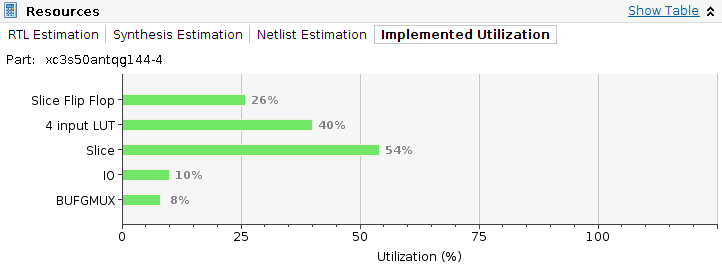
\includegraphics[width=\linewidth]{img/thresholding.png}
\caption{Logic consumption of project with a simple thresholding algorithm as decider}
\end{subfigure}

\end{figure}

\subsection{SPI}
The analog to digital converter (ADC) supplied by the supervisor uses a SPI protocol as it's form of communication, so a module in the FPGA needs to be set up.

\subsubsection{Protocol}
The FPGA will serve as the master and the ADC as the slave. In the VHDL module a clock is generated in order for the slave to have a signal on which to send data out, making the communication synchronous. The communication is full-duplex, and the master puts data out on it's wire (MOSI) before the falling edge of the serial clock, in order for the ADC to read it, which is done on the falling edge. The reverse is happening on the slave. It puts data out on it's wire (MISO) before the rising edge of the serial clock for the master to read on rising edge. The ADC does not sample continuously, but it has to be requested data. A request can be seen in figure \ref{time_spi_sample}. What is happening is that the master putting chip select (CS) low, and it sends a command to the ADC. The content of the command is a start bit, a configuration bit, which tells the ADC if it is running single or differential mode and 3 bits to select the channel. After this the status of the MOSI is \textit{don't care}. In order for the ADC to make the sample and hold, it needs the time of one clock cycle in order for the internal capacitor to charge, so after the last bit of the channel one clock cycle, nothing happens. After this cycle the data is clocked out. When the master has received 10 bits of data, CS is taken high and the clock is shut off.

\begin{figure}[h]
 \centering
 \begin{tikztimingtable}
  CLK	& H35{T}H\\
  CS	& H35{L}H\\
  MOSI	& LL2D{S}2D{S/D}6D{CH}25{U}\\
  MISO	& 14{Z}22D{ADC DATA}Z\\
 \end{tikztimingtable}
\caption{Timing diagram of taking one sample}
\label{time_spi_sample}
\end{figure}

\subsubsection{Implementation}
Given the datasheet \footnote{MCP3008,p1}
the maximum clock frequency of the SPI clock is $3.6$ MHz which gives a period time of 277 ns, but since this is not possible to obtain due to the system clock period being 20 ns. Taking the nearest number that to 277 that divides evenly with 20, 280, a clock frequency of $3.571$ MHz, which should be more than sufficient. Therefore a clock is generated with this period time in this VHDL module and put out on an output pin.

In order to keep the abstraction level, that this module is only for communication, it is the \textbf{LED\_driver} module that tells the \textbf{spi\_module} to initiate a sample. When a sample is received the data is just passed on to the LED\_driver, and a flag is set in order to tell the driver that new data has arrived.

\subsection{MotorControl}
In order to make the sorting happen, a servo motor with a mounted plastic rod is used. The colors that the \textbf{LED\_driver} has detected is fed in to the module, one wire for each color. The motor controller then decides which way the rod should point. If there are more than one color wire that is high, the rod is placed in the middle. 

The servo motor is controlled by a pulse width modulated (PWM) signal. The standard for RC-servo motors\footnote{Add reference to Electronics book}, one of which was provided for this project, a pulse width of 1 ms to be on the left extreme and 2 ms for the right extreme, with a PWM period of 20 ms. Since it is not needed to go to the extremes, some new width values has to be put in. It was found out that these values should be 1.35 ms to make the bricks slide right and 1.65 ms to make them slide left.

\subsection{$\mu$TosNet}
When working with an FPGA, especially with one with limited I/O pins, setting up some sort of user interaction is very limited and sometimes very primitive. This can be a problem if the system is complex. Therefore setting up communication with a PC could be a nice feature. This is where $\mu$TosNet come in to the picture. $\mu$TosNet uses UART, which is a serial communication using only 2 wires. This makes it good for non I/O heavy FPGA. 

In order to communicate with the FPGA a simple program has been written in C++, building on a skeleton found on the internet\footnote{\url{http://www.webalice.it/fede.tft/serial_port/serial_port.html}}. The program interfaces a simple UI where the user can input threshold values and then the program figures out what command should be sent. 
\subsubsection{Usage}
Due to the VHDL compiler being slow and tedious it could be nice to be able to change the thresholds of the different colors from the computer instead of compiling and flashing every time you want to fine tune the system. Another parameter that could be interesting to monitor is the current value of the ADC, in order to estimate what values could be good to use for the threshold. 


\newpage

\section{Tests}

\subsection{Power Supply} \label{sec:test_pwr_supply}

In order to test if the power supply works, each source was tested under load.
The tests are meant to simulate real use cases as prolonged test of the extreme loads might damage components and cause a setback.

The 5 V supply was tested with a constant load of $25 \Omega$, equivalent to the FPGA.
The voltage of the supply is held steady and within the $75 mV$ tolerance of 5 V.
The voltage can be seen in figure \ref{fig:5v_supply_test}.

\begin{figure}[h]
 \centering
 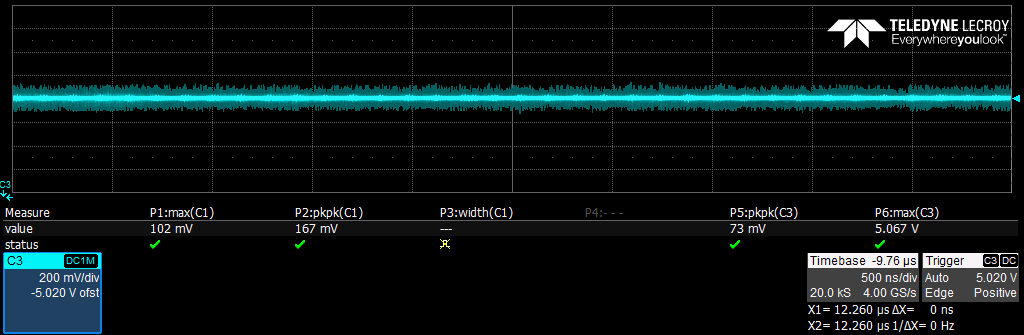
\includegraphics[width=0.9\linewidth]{img/5vsupply}
 \caption{5 V supply voltage test.}\label{fig:5v_supply_test}
\end{figure}

The 6 V supply was tested with the servo motor connected, receiving a change in pulse width, thus forcing the motor to rotate.
The voltage of the supply is held steady and within $400 mV$ tolerance of 6 V.
The voltage can be seen in figure \ref{fig:6v_supply_test}.

\begin{figure}[h]
 \centering
 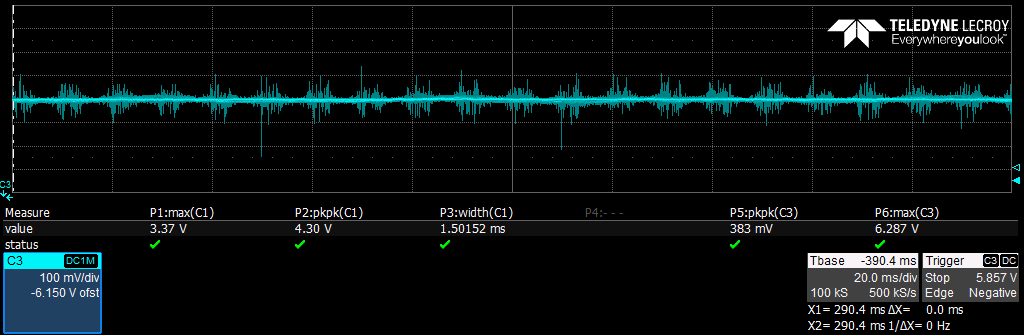
\includegraphics[width=0.9\linewidth]{img/6vsupply}
 \caption{6 V supply voltage test.}\label{fig:6v_supply_test}
\end{figure}


The 12 V supply was tested by using a turning a load on and off with a mosfet.
The load was a constant $120 \Omega$ resistor and the pulse was added from another $120 \Omega$ resistor, turned on an off with a mosfet.
This is meant to simulate the turning on and off of a diode.
In figure \ref{fig:12v_power_supply_voltage_test} can the step response from such a load be seen.

\begin{figure}[h]
 \centering
 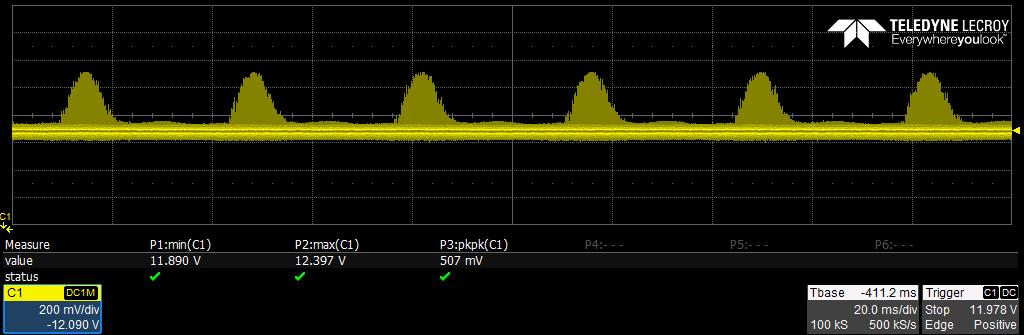
\includegraphics[width=0.9\linewidth]{img/power_test_12V_pulse}
 \caption{Step response of the 12 V supply with a changing load.}\label{fig:12v_power_supply_voltage_test}
\end{figure}




\subsection{Current test of photo diode}
This test was done in order to dimension the resistor for the operational amplifier (op-amp), for the amplification.
The desired range of the output of the amplifier is 0 to 3.3 V to make it directly correlated with the ADC, which is powered by 3.3 V. 
\subsubsection{Setup}
The photo diode is put in a breadboard and the current through is measured using a multi meter. The different colored LED's are set up with a resistor so that they draw 50 mA of current which is the max DC-current\cite{apnote:led}. The LED's and the photo diode are placed as they would on the final board, with a slight tilt towards the photo diode. A brick is then held over the diodes, and the current is read off the multi meter.
The setup can be seen in figure \ref{fig:photo_diode_current_setup}.

\begin{figure}[ht]
 \centering
  \begin{circuitikz}
  \node[ground,name=gnd] at (0,0) {}; 
  \draw
  (gnd) to ++(0,1) to[ammeter] ++(2,0) to[pD] ++(2,0) to[R] ++(2,0)  |- (gnd)
  ;
  \draw (0,2) node[left] {$12V$} to[short, o-] ++(2,0) to[leD,mirror] ++(2,0) to[R] ++(2,0) |- (gnd); 
  \end{circuitikz}
  \caption{Setup to measure current of photo diode.}
  \label{fig:photo_diode_current_setup}
\end{figure}

\subsubsection{Results}
The results of the test can be seen in table \ref{tab::test_pd}.
\begin{table}[H]
\centering
 \begin{tabular}{|c|ccc|}
 \hline
 \diagbox{LED}{Brick}
        & Red         & Green       & Blue          \\ \hline
  Red   & $16\ \mu A$ & $2\ \mu A$  & $5\ \mu A$    \\ 
  Green & $5\ \mu A$  & $13\ \mu A$ & $9\ \mu A$    \\
  Blue  & $5\ \mu A$  & $6\ \mu A$  & $19\ \mu A$   \\
  \hline
 \end{tabular}
\caption{Outcome of the test}
\label{tab::test_pd}
\end{table}

Dividing $1 V$ with $10 \mu A$ in order to get the order of magnitude, gives $100 000$. This leads to the value of the resistor should be $100 k\Omega$.
This was tested to be accurate with the setup in figure \ref{fig:photo_diode_voltage_setup}.


\subsubsection{Conclusion}
Given the results of the test it was decided that a value of $100 k\Omega$ would be a reasonable. This gives $0.1 \frac{V}{\mu A}$.

\subsection{Rise time test of amplifier} \label{sec:rise_time_test}

The purpose of this test is to test the rise time of the amplifier to see if it can handle fast changes on the input.

It is expected that the load of the op-amp is not an ideal resistance. 
Due to the fact that we are not dealing with an ideal op-amp and the circuit introduces capacitance, the amplifier has a capacitive load. 
The feedback resistor is large enough so the circuit can be simplified by reducing it to a RC circuit.
A capacitor will always try to minimize the change in voltage, so with a high frequency of switching, the voltage will oscillate. To test the extend of this oscillation, a test setup without compensation is created.
\begin{wrapfigure}{r}{0.49\linewidth}

 \centering
  \begin{circuitikz}[scale=\figscale, every node/.style={scale=\figscale}]
  %opamp part
  \node[op amp,name=G] at (0,0) {}; 
  \node[ground,name=gnd] at ($(G.+)+(-3,-1)$) {}; 
  \draw
  (gnd) -| (G.+) 
  (gnd) to[short] ($(G.-)+(-3,0)$) to[pD] ($(G.-)+(-0.5,0)$) node[name=intersection] {} to (G.-)
  (G.out) to ++(0,1.5) coordinate(Rright) to[R=$100K\Omega$] ++(-2.7,0)  -| (intersection.center) coordinate(Rleft)
  (G.out) to[short,-o] ++(1,0) node[right,name=out] {$V_{out}$} 
  (out.west) to[voltmeter] ++(0,-1.5) -| (gnd) 
  ;
  \draw (Rleft) |- ++(1,2) to[C=$C_f$] ++(1,0) -| (Rright);
  %led part
  \node[nmos, name=mosfet,rotate=-90] at (-3,3.5) {};
  \draw (mosfet.S) -| (gnd) 
  (mosfet.D) to[leD] ++(2,0) to[R=$160\Omega$] ++(2,0) to[short,-o] ++(1,0) node[right] {$12 V$}
  (gnd) |- ($(mosfet.G)+(0,1)$) to[sqV] (mosfet.G) 
  ;
  \end{circuitikz}
  \caption{Setup to measure voltage of photo diode.}
  \label{fig:photo_diode_voltage_setup}
 \end{wrapfigure}


A red diode was used for the test, so the expected output voltage is $2 V$.
To test for ringing effect the naive setup, shown in figure \ref{fig:naive_voltage},
is used to see if the op-amp can keep up with a high speed signal.\
This resulted in a ringing effect and thus the signal could not settle before the diode is turned off again.
\matthias{undefined ref. ved ikke lige til hvad}
In figure \ref{fig:scope_op_amp_no_C} can this effect be seen.

\begin{figure}[t]
\centering
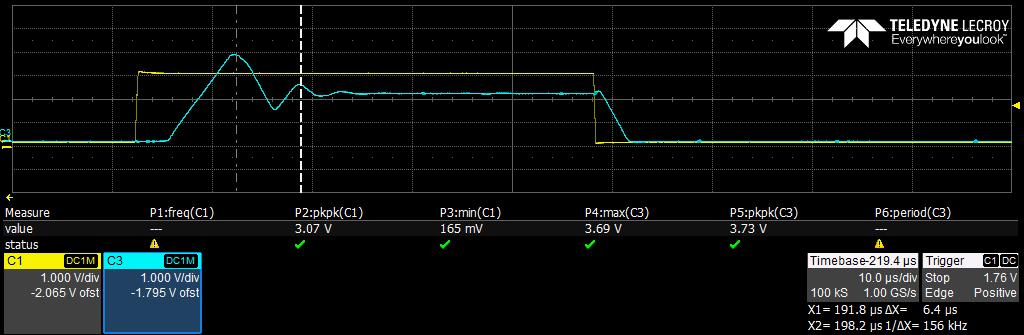
\includegraphics[width=0.9\linewidth]{img/amp_test_ringing2.jpg}
\caption[Ringing effect of amplifier.]{Ringing effect of amplifier. The yellow line shows when the LED is turned on and off, and the blue is the output of the amplifier}
\label{fig:scope_op_amp_no_C}
\end{figure}

The communication with the ADC is $3.6 MHz$. 
With a message size of $18$ bits this means it will be sampling at $190 kHz$.
To give the amplifier time to settle the ADC will be read three times, throwing away the results from the first two samples.
This effectively gets the frequency down to $63 kHz$ and reading becomes possible.
For simplicity the LED signal will be treated as a $63 kHz$ pulse in this section.
% 
% \begin{figure}[ht]
% \centering
% \begin{tikztimingtable}[xscale=0.3]
%  slow\_clk       & L12{2{T}}2{19{2{T}}}15{2{T}}\\
%  led\_signal     & Z 3{38D{R}} 1{15D{G}} \\
%  adc\_read       & 3{5{2L}2{2H}11{2L}1{2L} } 8{2L}\\
%  adc\_transfer   & {2L} 3{7{2L}1{20D{adc}} 1{2L}1{2L} } 7{2L}\\ 
%  sample\_done    & L18{2L} 2{1{2H}18{2L}} 1{2H}8{2L}\\ 
%  \extracode
%     \vertlines[dashed]{92,112} %8 clock cycles
% \end{tikztimingtable}
% \caption{Timing table of communication between the ADC and the FPGA. The interval is the data that is actually used. The rest of the data is just overwritten without being used.}\label{fig:communication_dummyreads}
To avoid the ringing effect, a capacitor is added as seen in figure \ref{fig:photo_diode_voltage_setup}.
To find a proper capacitance, equation \ref{eq:capacitance_approximate}\cite[p. 2]{art:cap}
is used to find an approximate.
The frequency, $f$, is found by measuring the period on the naive signal.
The period was found to be between $6$ and $7$ $\mu S$.
The capacitance estimate is thus between $9.55$ and $11.1 pf$. 
A feedback capacitor of $10 pf$ was chosen.

\begin{equation}
 C_f = \frac{1}{2 \pi f R_f} \label{eq:capacitance_approximate}
\end{equation}

In figure \ref{fig::scope_op_amp_with_C}, it can be seen that the amplifier now is critically damped and thus able to settle at a higher frequency.
The signal must be settled in the time the ADC measures, which is $560 ns$ from the falling edge of the chip select.
As it can be seen, the signal is readable at $65 kHz$.


\begin{figure}[h]
\centering
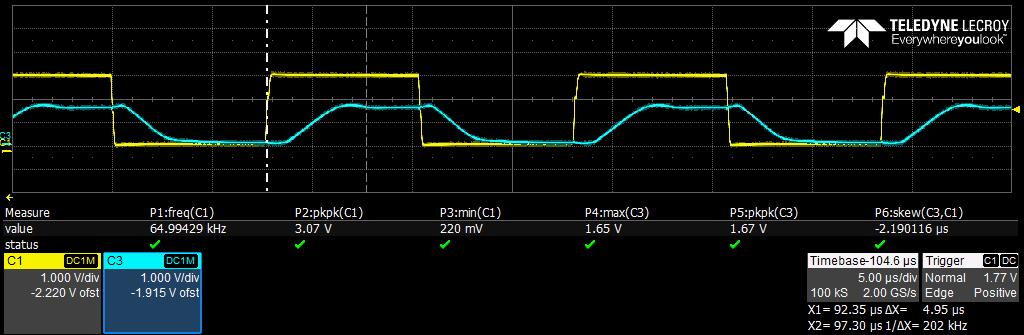
\includegraphics[width=0.9\linewidth]{img/ringing_test_filtered_rise.jpg}
\caption[Ringing effect of amplifier filtered.]{Ringing effect of amplifier filtered. The yellow line shows when the LED is turned on and off, and the blue is the output of the amplifier}
\label{fig::scope_op_amp_with_C}
\end{figure}

\subsection{ADC}
To test if the ADC works with the FPGA, the ADC was tested on a breadboard.
A controlled input was given to the ADC and the MISO signal was analyzed to find the ADC value.
The ADC value is a the last 10 bits of the 17 bit package on the MISO, sent after a falling edge on the CS.
In figure \ref{fig:scope_adc} is the oscilloscope readings for a test with 2.1 V input shown.

To see how the ADC handles the input voltage a series of measurements has been made with a 0.1 V step between measurements.
Figure \ref{fig:adc_values} shows the ADC values in decimal in relation to the input voltage.
From this it can be seen that the ADC values are proportional to the input voltage and thus the ADC communication works.
The data code for the data processing can be found in appendix \ref{app:adc_R_code}.

\begin{figure}[ht]
 \centering
 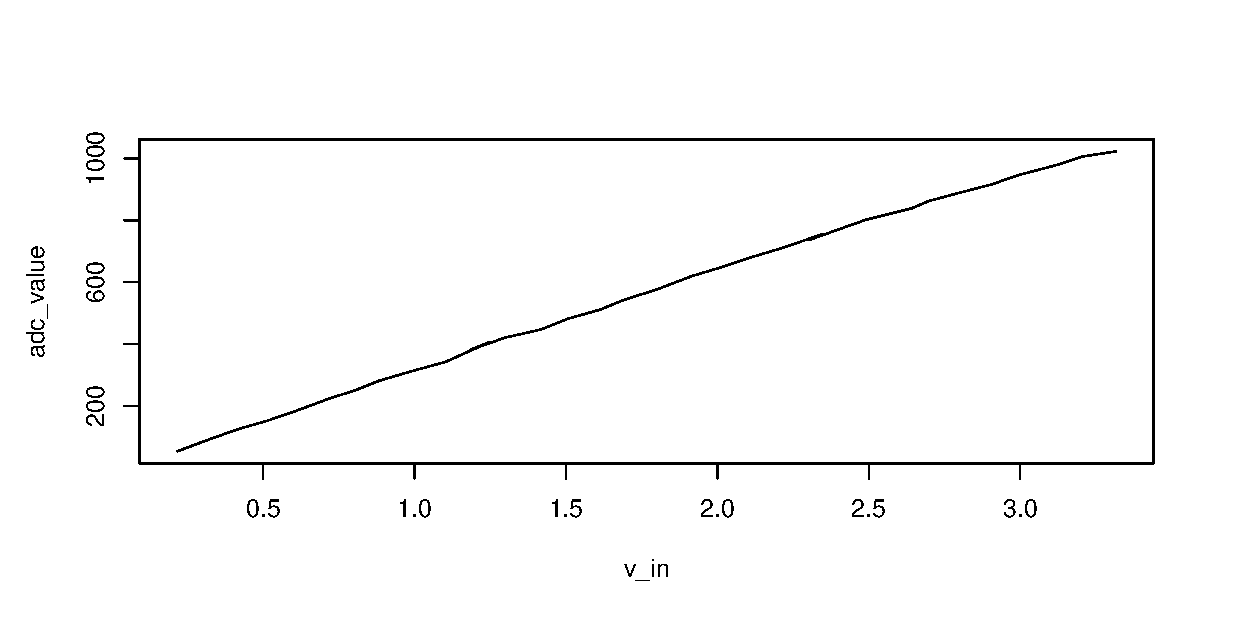
\includegraphics[width=0.7\textwidth]{img/ADC_values}
 \caption{ADC values in relation to input voltage.}
 \label{fig:adc_values}
\end{figure}

\begin{figure}[ht]
    \centering
    \begin{tikzpicture}
        \node {
        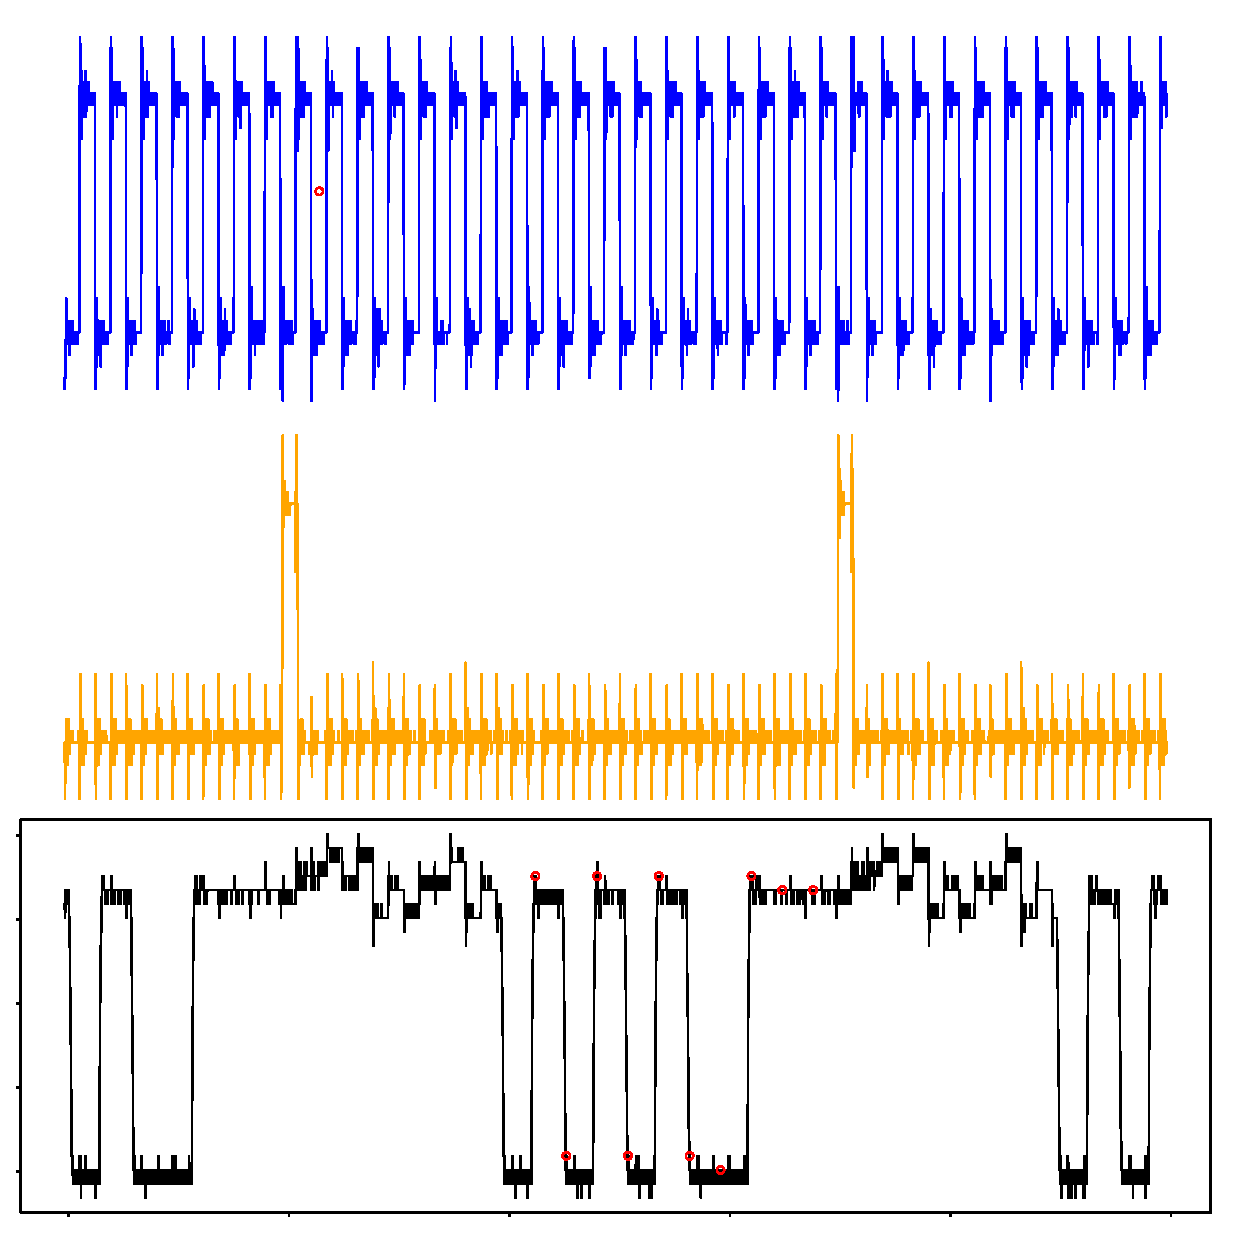
\includegraphics[width=0.7\textwidth]{img/scope_adc} 
        };
        \node at (-6.5,4)  {CLK};
        \node at (-6.5,0)  {CS};
        \node at (-6.5,-4) {MISO};
    \end{tikzpicture}
    \caption[Oscilloscope measurements for ADC]
            {Oscilloscope output of the ADC connections for the 2.107 V RMS input. The red dots signify when the signal is read.}
            \label{fig:scope_adc}
\end{figure}

% the figures I like is BACK
\begin{figure}[h]
\centering
\begin{tikztimingtable}[xscale=0.3]
 slow\_clk       & L2{26{2{T}}          }L\\
 led\_signal     & Z 1{50D{R}}1{2Z} 1{50D{G}}1{2Z}      L\\
 adc\_read       & L2{13{2L}2{2H}11{2L} }L\\
 adc\_transfer   & L2{15{2L}10{2H}1{2L} }L\\
 signal\_complete& L2{25{2L}1{2H}       }L\\
\end{tikztimingtable}
 \caption{ADC communication, naive approach.}\label{fig:naive_communication}
\end{figure}

\begin{figure}[h]
\centering
\begin{tikztimingtable}[xscale=0.3]
 slow\_clk       & L12{2{T}}3{19{2{T}}          }\\
 led\_signal     & Z 1{38D{R}} 1{38D{G}}1{38D{B}} 1{24D{R}} \\
 adc\_read       & L12{2L} 3{5{2L}2{2H}11{2L}1{2L} }\\
 adc\_transfer   & L12{2L} 3{7{2L}1{20D{adc}}1{2L}1{2L} }\\ 
 sample\_done    & L29{2L} 2{1{2H}16{2L}     2{2L} }1{2H}LL\\ 
 \extracode
    \vertlines[dashed]{61,77,99,115} %8 clock cycles
\end{tikztimingtable}
\caption{ADC communication optimized.}\label{fig:optimized_communication}
\end{figure}


\bibliographystyle{ieeetr}
\bibliography{src/bibtex}

\matthias{Bill of materials}
\end{document}
